\documentclass{article}
\usepackage[a4paper, left=1in, right=1in, top=1in, bottom=1in]{geometry}
\usepackage{graphicx}
\usepackage{pgfplots}
\usepackage{multirow}
\usepackage{booktabs}
\usepackage{longtable}
\pgfplotsset{compat=1.17}
\usepackage{tabularx}
\usepackage{booktabs}
\graphicspath{{./images/}}
\usepackage{siunitx}
\usepackage{tikz}
\usepackage{array}
\usepackage{xcolor}
\usepackage{pdflscape}
\usepackage{soul}
\definecolor{lightyellow}{rgb}{1,1,0.7}
\sethlcolor{lightyellow}
\usepackage{amsmath}
\usepackage{float}
\usepackage{hyperref}
\usepackage{subcaption}
\usepackage{tocloft} 

\setlength{\parindent}{0pt}
\usepackage[utf8]{inputenc}

\begin{document}
\tableofcontents
\newpage

\section{World Beverage Market}
The analysis of the market, including the \textbf{existing beverage market, market segments related to freshwater, and the overall Target Market} are pivotal considerations in the inception phase of our Bahama project, especially when considering the establishment of a bottling factory. The essence of gauging market demand lies in its direct correlation with the salability of our product. Regardless of the production capacity or product quality, the project’s success hinges on our ability to sell the product effectively in the targeted market. Hence, a thorough market demand analysis is indispensable to avoid unfavorable outcomes and to ensure that our investment in the Bahamas project yields a positive return. \par

The global beverage market is vast and diverse, encompassing various drink types, including soft drinks, juices, tea, coffee, and bottled water. Major players in this market significantly impact consumer choices, market trends, and the overall landscape of the beverage industry. First, we present the market growth projection from 2022 to 2030, as surveyed by CAGR: \href{https://www.mordorintelligence.com/industry-reports/beverages-market}{Click here for the Source}.
\begin{figure}[H]
\centering
\includegraphics[width=12cm]{图片8888.png}
\label{fig:unique_label_1}
\caption{CAGR Market Growth Data}
\end{figure}
\begin{figure}[H]
\centering
\includegraphics[width=8.5cm]{35.png}
\label{fig:unique_label_1}
\end{figure}
\subsection{Major Companies, Market Segments, and Juice types}
The beverage market is dominated by several large corporations that have a global presence. Some of these include: \textbf{The Coca-Cola Company, PepsiCo,Nestlé, Danone, and Keurig Dr Pepper.}\par

The market can be broadly divided into several segments, such as: \textbf{Carbonated Soft Drinks, Juices and Smoothies, Bottled Water, Tea and Coffee, and Energy and Sports Drinks.}\par

Among the non-alcoholic beverage sector, juices hold a significant share. Key types of juices include:
\textbf{Orange Juice, Apple Juice, Grape Juice, Tropical and Mixed Fruit Juices, Vegetable Juices.}\par

The market share varies by region and segment. For example, carbonated drinks have a higher market share in North America, while tea and coffee dominate in Asia. The global beverage market continues to evolve, with trends like health-conscious products and sustainable packaging influencing future developments.
\begin{table}[h]
\centering
\begin{tabularx}{\textwidth}{|>{\centering\arraybackslash}X|>{\centering\arraybackslash}X|}
\hline
\textbf{Market Segment} & \textbf{Description} \\ \hline
Carbonated Soft Drinks & Beverages that are carbonated and typically sweetened, flavored, and non-alcoholic. \\ \hline
Juices & Beverages made from the extraction or pressing of the natural liquid contained in fruits and vegetables. \\ \hline
Bottled Water & Drinking water sold in bottles, including mineral water, spring water, and purified water. \\ \hline
Tea and Coffee & Hot beverages made by steeping tea leaves or coffee beans, available in various flavors and preparations. \\ \hline
Energy and Sports Drinks & Beverages designed to boost energy, improve athletic performance, and replenish electrolytes. \\ \hline
Alcoholic Beverages & Beverages containing ethanol, including beer, wine, and spirits. \\ \hline
Dairy Beverages & Milk-based drinks, including flavored milk, yogurt drinks, and others. \\ \hline
\end{tabularx}
\caption{Key Segments of the World Beverage Market}
\label{table:beverage_market_segments}
\end{table}

\subsection{World Bottled Water Market}
\subsubsection{Questions we raise}
\begin{itemize}
    \item \textbf{How big is the bottled water market?}
    \item \textbf{What is the bottled water market growth?}
    \item \textbf{Which segment accounted for the largest bottled water market share?}
    \item \textbf{Who are the key players in the bottled water market?}
    \item \textbf{What are the factors driving the bottled water market?}
\end{itemize}

\subsubsection{Adress the questions}
\begin{itemize}
    \item \textbf{Global Market Size in 2022:} The market was estimated at approximately USD 303.95 billion. It is projected to grow at a compound annual growth rate (CAGR) of 5.9\% from 2023 to 2030.
    \item \textbf{Growth Drivers:} The increase is primarily driven by health concerns such as gastrointestinal diseases linked to contaminated water and the scarcity of safe drinking water in various regions. Additionally, the rising preference for nutrient-fortified water due to increased health consciousness among consumers is a significant factor.
    
\end{itemize}
\begin{figure}[H]
\centering
\includegraphics[width=\linewidth]{4.png}
\label{fig:unique_label_1}
\end{figure}

\textbf{Market Segments}\par
\begin{itemize}
    \item \textbf{Still Water Segment:} In 2022, still water held the largest market share of more than 74.5\% in revenue terms, dominating the market due to consumer preference for safe and clean drinking options.
    \item \textbf{Functional Water Segment:} This segment is expected to register the fastest CAGR of 6.9\% from 2023 to 2030, driven by growing consumer awareness of health and wellness and the demand for beverages that support specific health goals.
\end{itemize}

\textbf{
Distribution Channels}\par
\begin{itemize}
    \item \textbf{Off-trade Segment:} dominated the market with a revenue share of over 88.8\% in 2022, including retail outlets like supermarkets and convenience stores.
    \item \textbf{On-trade Channel:} Anticipated to grow rapidly with the fastest CAGR of 10.1\% from 2023 to 2030, benefiting from social and recreational activities in restaurants and entertainment venues.
\end{itemize}
\textbf{Packaging}\par
\begin{itemize}
    \item \textbf{PET Segment:} accounted for the largest revenue share of more than 80.0\% in 2022, favored for its cost-effectiveness and reduced transportation costs.
    \item \textbf{Cans Segment:} Projected to register rapid growth with a CAGR of 6.4\% from 2023 to 2030, offering superior product protection and ensuring freshness and purity.
\end{itemize}
\begin{figure}[H]
\centering
\includegraphics[width=\linewidth]{2.png}
\label{fig:unique_label_2}
\end{figure}
\textbf{Key Companies}
\begin{itemize}
    \item \textbf{Major Players:} Include \textbf{Nestlé, PepsiCo, The Coca-Cola Company}, DANONE, among others. These companies are focusing on strategies like new product launches and global expansions.
\end{itemize}
\begin{figure}[H]
\centering
\includegraphics[width=8cm]{5.png}
\label{fig:unique_label_5}
\caption{Four Major players worldwide}
\end{figure}

\begin{table}[H]
\centering
\small
\begin{tabularx}{\textwidth}{|>{\centering\arraybackslash}X|>{\centering\arraybackslash}X|>{\centering\arraybackslash}X|>{\centering\arraybackslash}X|>{\centering\arraybackslash}X|}
\hline
\textbf{Company Name} & \textbf{Est. Market Share Ratio} & \textbf{Product Types} & \textbf{Price Range} & \textbf{Remarks} \\ \hline
Nestlé & High & Pure Water, Functional Water, etc. & \$ - \$\$ & Diverse products, widespread global presence \\ \hline
PepsiCo & Medium & Sparkling Water, Pure Water, etc. & \$ - \$\$ & Significant growth in functional water market \\ \hline
The Coca-Cola Company & Medium & Sparkling Water, Pure Water, etc. & \$ - \$\$ & Variety of products, focuses on brand image \\ \hline
DANONE & Medium & Pure Water, Mineral Water, etc. & \$ - \$\$\$ & Emphasizes health and environmental attributes \\ \hline
FIJI Water Company LLC & Small & Natural Mineral Water & \$\$ - \$\$\$ & Premium market, emphasizes purity and naturalness \\ \hline
Gerolsteiner Brunnen GmbH \& Co. KG & Small & Natural Mineral Water & \$\$ - \$\$\$ & Focuses on the European market, premium positioning \\ \hline
VOSS WATER & Small & Premium Mineral Water & \$\$\$ & Ultra-premium market positioning, focus on brand image \\ \hline
Nongfu Spring & Large in Asia & Pure Water, Mineral Water, etc. & \$ - \$\$ & Leading position in the Chinese market \\ \hline
National Beverage Corp. & Small & Sparkling Water, Pure Water, etc. & \$ - \$\$ & Holds a certain market share in North America \\ \hline
Keurig Dr Pepper Inc. & Small & Various beverage products & \$ - \$\$ & Diverse product range, covers multiple beverage markets \\ \hline
\end{tabularx}
\caption{Major Bottled Water Companies and Their Price Points}
\label{table:bottled_water_companies}
\end{table}

\subsubsection{Regional Insights}
\textit{\textbf{Asia Pacific}}\par
Asia Pacific made the largest contribution to the global market with a revenue share of 45.1\% in 2022. Growing awareness about the importance of health and wellness in countries including China, India, Malaysia, and Indonesia is one of the major factors supporting the market growth owing to the heightened demand for hygienic consumables. With the growing awareness about the importance of hygienic beverage options, the demand for bottled options is also increasing, thereby creating avenues for the bottled water market growth in the region.\href{https://www.grandviewresearch.com/industry-analysis/bottled-water-market}{(Source)}

\textit{\textbf{United States}}\par
In the United States, the bottled water market has hit new peaks in both volume and sales as of 2022, showcasing a growing preference for bottled water among consumers. The market value was reported at USD 22.175 billion in 2021 and is expected to grow at a Compound Annual Growth Rate (CAGR) of 8.42\% from 2022 to 2030. The overall market size for bottled water in the US is expected to grow from USD 316.76 billion in 2023 to USD 426.70 billion by 2028, at a CAGR of 6.14\% during the forecast period (2023-2028). North America made the second-largest contribution to the global market with a revenue share of 23.9\% in 2022. The growing trend of living a healthy lifestyle and extensive sports and other physical and outdoor activities are also responsible for the high demand for bottled water. Most Americans do not prefer drinking water straight from the tap as they find packaged options to be a safer and more convenient option. Moreover, the rising demand for eco-friendly and sustainable packaging solutions by customers is expected to offer lucrative opportunities for existing manufacturers and new entrants in the market. In 2022, the U.S. accounted for 57.7\% of the market share. People are now more conscious about their health and are realizing the significance of consuming nutritious beverages. Bottled water is being recognized as a better choice compared to sugary drinks.\href{https://www.grandviewresearch.com/industry-analysis/bottled-water-market}{(Source)}

\textit{\textbf{Caribbean}}\par
The revenue in the Bottled Water segment in the Caribbean amounts to USD 1.76 billion in 2023, with an expected annual growth rate of 4.89\% (CAGR 2023-2027). However, the Latin American bottled water market (which includes the Caribbean) saw a modest decline in 2022, waning by -2.2\% against the previous year, which might reflect regional variations in market trends. The bottled water market in both the US East and the Caribbean region is exhibiting growth, albeit with different market dynamics and growth rates.

\textit{\textbf{Europe}}\par
Europe is expected to grow at a CAGR of 5.2\% from 2022 to 2030. The tourism industry plays a significant role in driving the demand for the market in Europe. With millions of tourists visiting European countries each year, the need for reliable and safe drinking water is essential. Bottled water offers a convenient solution for both domestic and international tourists who may be unsure about the quality of tap water in unfamiliar destinations. Germany is expected to grow at a CAGR of 5.7\% during the forecast period. The market is poised for growth primarily due to increasing awareness among individuals about the significance of maintaining proper hydration. Moreover, there is a rising demand for premium bottled water as people seek healthier options. Furthermore, the fact that consumers now have higher disposable incomes adds to the expansion of the market.\href{https://www.grandviewresearch.com/industry-analysis/bottled-water-market}{(Source)}
\begin{figure}[H]
\centering
\includegraphics[width=\linewidth]{1.png}
\label{fig:unique_label_3}
\end{figure}

\begin{figure}[H]
\centering
\includegraphics[width=\linewidth]{3.png}
\label{fig:unique_label_4}
\end{figure}

\section{Demand Analysis Local | Regional | International}
\subsection{Local Demand}
The local population of the Bahamas also forms a key part of the target market for bottled water. Many Bahamians may prefer bottled water for its convenience and perceived purity, particularly where tap water quality is a concern. Also, the UN predicts a slight growth in the population of the Bahamas until 2048 and will have a decreasing trend from 2048 to 2100. There is no significant growth in the total population. However, due to the little marginal revenue of the traditional plastic bottled water (average price of \$1 per bottle), \textbf{the locals might not become our major source of income.} 

\begin{figure}[H]
\centering
\includegraphics[width=\linewidth]{7.png}
\caption{Historical demographics of The Bahamas }
\label{fig:unique_label_8}
\end{figure}

\subsubsection{Tourists and Visitors}
The Bahamas is an international tourist destination with visitors from around the world. The USA is the largest tourist contributor making up  80\% of the visitors. Historical data shows that March will be the month with the highest number of visitor arrivals, while in September there are the fewest tourists. (Source? Footnote/endnote?) 

\begin{figure}[H]
\centering
\includegraphics[width=\linewidth]{8.png}
\caption{The Bahamas Visitor Data 2010-2023 Based on Island}
\label{fig:unique_label_8}
\end{figure}

The aggregated data from 2010 to September 2023 shows / suggests that New Providence Island became the largest tourist attraction with 54\% contributors, followed by The \textbf{Out Islands | Family Islands (to which Andros belongs) with 35\% and Grand Bahama by 11\%}. The pie chart below shows the tourist distribution between the three islands. 

\begin{figure}[H]
\centering
\includegraphics[width=13cm]{9.png}
\caption{Proportion of visitors on each Island}
\label{fig:unique_label_9}
\end{figure}

Andros does not attract the most tourists, as shown by the monthly visitor lists over the last 13 years. Based on this aggregated data, from the total number of tourists, who came to the Bahamas, only 0.17\% visited Andros. However, Andros is the major island of The Bahamas in respect to size and in respect to readily available freshwater. In order to protect through a social, environmental, and economic beneficial stewardship program this pressures the natural resource of Andros. \textbf{The intent is to choose Andros Island as our base for the sourcing and distribution of “BA Water” to The Bahamas islands, the region, and the world. }

\begin{table}[h]
\centering
\begin{tabular}{lcc}
\toprule
Total Bahamas & Andros & \% \\
\midrule
79,743,042 & 138,830 & 0.17\% \\
\bottomrule
\end{tabular}
\caption{Andros Proportion}
\label{tab:my_table}
\end{table}

\begin{figure}[H]
\centering
\includegraphics[width=13cm]{10.png}
\caption{Andros Visitor Data 2010 - 2023 Based on Island}
\label{fig:unique_label_10}
\end{figure}




\subsubsection{The Predictive Trend on Visitors}  

The Bahamas suffered significant financial loss due to the pandemic as their main industry is tourism, but they bounced back fast and the 2023 year-to-date data already shows positive trends compared to the pre-pandemic area.\par
Tourism in the Bahamas for the upcoming years forecasts a growth trend. Estimated tourist trend for the next 20 years based on the last 10 years’ historical data excluding the pandemic area, shows that the estimated visitor per month in the Bahamas area, the maximum, minimum, and average visitor per month per year have a distribution as follows. (Source – footnote where the data is coming from.) \par

\begin{table}[h]
\centering
\begin{tabular}{lc}
\toprule
Statistic & Value \\
\midrule
Max & 975,863 \\
Min & 597,501 \\
Average & 805,389.8 \\
\bottomrule
\end{tabular}
\caption{Different Scenarios}
\label{tab:statistics}
\end{table}

\begin{figure}[H]
\centering
\includegraphics[width=\linewidth]{11.png}
\caption{Different Scenarios }
\label{fig:unique_label_11}
\end{figure}

From the literature review, \textbf{almost 70\% Bahamas visitors a day visitor, and stop-over visitors contribute to the remaining 30\%,} the stop-over visitors’ expected stays in the islands are around 7 days on average, which gives the next point of view: 

\subsubsection{The Cruise Ships} 
Securing business with cruise ship companies entails extensive effort, communication, and negotiation. The Bahamas welcomed \hl{\textbf{over 3.2 million}} cruise passengers in 2022, with hopes of increasing this number to over 4 million in 2023. The average capacity of ocean liners, which are the primary type of cruise ships visiting the Bahamas, is around 3,000 guests. Since the restart of cruising in 2021, the Nassau Cruise Port has received 1,592 cruise ship calls.\par

\begin{figure}[H]
\centering
\includegraphics[width=\linewidth]{12.jpg}
\caption{The Bahamas Cruise Ships}
\label{fig:unique_label_11}
\end{figure}
Assuming an average capacity of 3,000 passengers per ship and 3.2 million cruise passengers in a year. \hl{Cruise passengers would constitute approximately \textbf{52.20\% }of the total tourists}.\textbf{The estimated annual number of cruise ships visiting the Bahamas is approximately 1,067.} That gives us a strong hint that it would be advantageous if our project could directly engage with the cruise ship companies to discern their potential demand and explore the feasibility of sourcing from a local bottling plant.

\subsubsection{Conclusion Market and Market Segment Analysis }
The data shows the expected market for normal bottled water in the Bahamas every year, \textbf{including the stops by tourists(cruise ships, hotels), the local population, and long-term visitors):} 

\begin{figure}[H]
\centering
\includegraphics[width=\linewidth]{13.png}
\caption{Bahamas Market (Tourist \& Population) }
\label{fig:unique_label_11}
\end{figure}

\begin{figure}[H]
\centering
\includegraphics[width=\linewidth]{14.png}
\caption{Estimated Monthly Demand}
\label{fig:unique_label_11}
\end{figure}

Estimated Daily Demand uses March data as the highest tourist arrivals and September as the lowest tourist arrivals. \textbf{The target market ranges from 468K to 480K people per day. }

\begin{figure}[H]
\centering
\includegraphics[width=\linewidth]{15.png}
\caption{Estimated Monthly Demand}
\label{fig:unique_label_15}
\end{figure}

\subsection{Regional Demand}
\subsubsection{United States}
\begin{itemize}
    \item Market Overview
\end{itemize}
The United States bottled water market, valued at USD 22.175 billion in 2021, is expected to grow at a CAGR of 8.42\% from 2022 to 2030. This growth is driven by a shift in consumer preferences towards healthier beverage options and a growing distrust in tap water quality.\par

\begin{itemize}
    \item Consumer Trends
\end{itemize}

The demand is further fueled by a lifestyle trend that emphasizes health and fitness, where bottled water is seen as a vital component. The rise in outdoor and sports activities also contributes to the increased consumption of bottled water.\par

\begin{itemize}
    \item Sustainable Packaging
\end{itemize}
An emerging trend in the market is the demand for eco-friendly packaging solutions. This presents an opportunity for innovation in sustainable packaging, potentially attracting a new segment of environmentally conscious consumers.\par

\begin{itemize}
    \item Forecast
\end{itemize}
Considering these factors, the market size is projected to expand from USD 316.76 billion in 2023 to USD 426.70 billion by 2028, growing at a CAGR of 6.14\%.\par

\subsubsection{Caribbean}\par
\begin{itemize}
    \item Current Market State
\end{itemize}

The Caribbean bottled water market is projected to reach USD 1.76 billion in 2023, with a CAGR of 4.89\% from 2023-2027. However, the market experienced a slight decline of -2.2\% in 2022, suggesting variable regional trends.\par

\begin{itemize}
    \item Regional Variations
\end{itemize}
The decline in the Latin American bottled water market, which includes the Caribbean, indicates a need for a deeper understanding of region-specific preferences and economic factors.\par

\begin{itemize}
    \item Opportunities and Challenges
\end{itemize}
The market dynamics in the Caribbean are influenced by tourism, climate, and local infrastructure. Bottled water is a necessity for tourists who prefer safe and reliable drinking options. However, environmental concerns and the need for sustainable practices present both a challenge and an opportunity for market players.\par

The analysis suggests \textbf{robust growth potential} in the United States, driven by health trends and sustainability initiatives. In contrast, the Caribbean market, while growing, requires a \textbf{tailored approach considering its unique regional characteristics} and the impact of external factors such as tourism and environmental concerns.

\subsection{International Demand}

\subsubsection{Asia Pacific}

The Asia-Pacific bottled water market is showing significant growth, with an expected increase from USD 84.47 billion in 2023 to USD 111.50 billion by 2028, at a CAGR of 5.71\%. Key factors contributing to this growth include rising health awareness and a preference for hygienic consumables.

\begin{figure}[H]
\centering
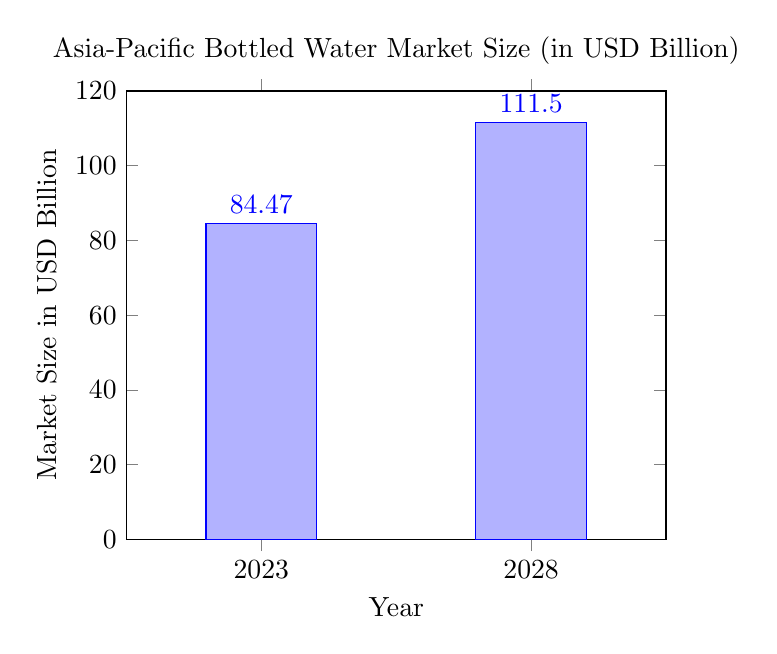
\begin{tikzpicture}
\begin{axis}[
    title={Asia-Pacific Bottled Water Market Size (in USD Billion)},
    xlabel={Year},
    ylabel={Market Size in USD Billion},
    symbolic x coords={2023, 2028},
    xtick=data,
    ybar,
    bar width=40pt,
    ymin=0, 
    ymax=120, 
    nodes near coords,
    nodes near coords align={vertical}, 
    enlarge x limits=0.5 
]
\addplot coordinates {(2023, 84.47) (2028, 111.50)};
\end{axis}
\end{tikzpicture}
\caption{Projected growth of the Asia-Pacific bottled water market from 2023 to 2028}
\end{figure}

\subsubsection{Europe}

Europe's bottled water market is expected to grow at a CAGR of 5.2\% from 2022 to 2030. The tourism industry significantly contributes to this growth.
\begin{itemize}
    \item Market Share by Region
\end{itemize}
A comparative analysis of market share by region shows the dominance of Asia Pacific, followed by North America (United States), Europe, and the Caribbean.

\begin{figure}[H]
\centering
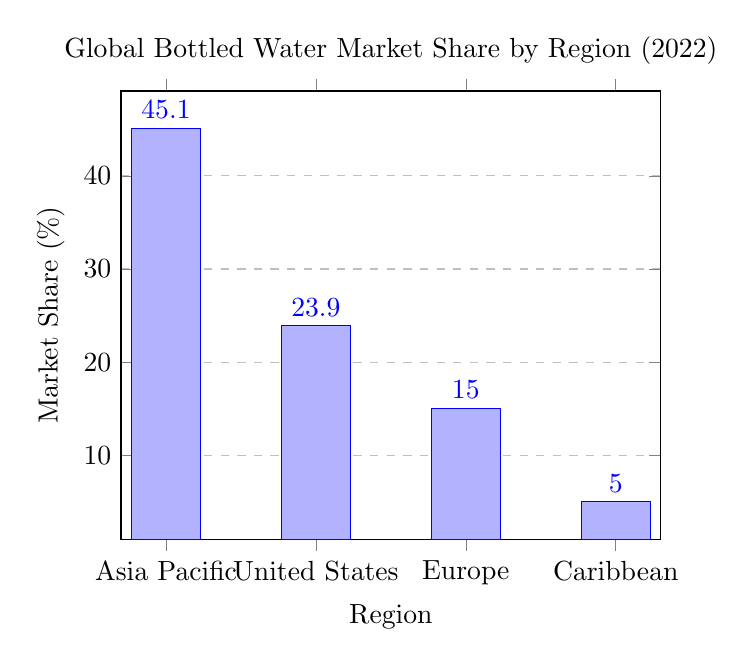
\begin{tikzpicture}
\begin{axis}[
    title={Global Bottled Water Market Share by Region (2022)},
    xlabel={Region},
    ylabel={Market Share (\%)},
    symbolic x coords={Asia Pacific, United States, Europe, Caribbean},
    xtick=data,
    ybar,
    bar width=25pt, % Adjusted bar width
    enlarge x limits=0.1, % Adjust the space between bars
    nodes near coords,
    nodes near coords align={vertical},
    ymajorgrids=true,
    grid style=dashed,
]
\addplot coordinates {(Asia Pacific,45.1) (United States,23.9) (Europe,15) (Caribbean,5)};
\end{axis}
\end{tikzpicture}
\caption{Bottled Water Market Share by Region in 2022}
\end{figure}

% European Market Data Table
\begin{table}[H]
\centering
\begin{tabular}{|l|l|}
\hline
\textbf{Market Size (2023)} & USD 70.20 billion \\
\textbf{Expected Size (2028)} & USD 84.30 billion \\
\textbf{CAGR (2023-2028)} & 3.73\% \\
\hline
\end{tabular}
\caption{Key Data of the European Bottled Water Market}
\end{table}

\begin{itemize}
    \item Conclusion
\end{itemize}
The international bottled water market shows diverse growth patterns across regions. Asia Pacific remains the leader, with significant potential in the United States and Europe. The Caribbean market, while smaller, presents unique opportunities due to its tourism-driven demand.


\subsection{Demand Seasonality}
Taking the assumption that each person needs 2 liters (0.5 gallons) as drinking water per day, we can infer that the daily demand for bottled water is substantial, with estimates ranging from around \hl{\textbf{ 935,662 to 960,073 liters}}. This suggests a significant market size and consumption rate for bottled water. Based on the seasonal adjustments, we can give a result of the total daily demand and the factories needed to fulfill:

\begin{table}[H]
\centering
\begin{minipage}{0.45\linewidth}
\centering
\begin{tabular}{@{}lS[table-format=7.0]S[table-format=2.0]@{}}
\toprule
{Month} & {Total Daily Demand (Liters)} & {Factories} \\
\midrule
January  & 859053 & 9 \\
February & 869424 & 9 \\
March    & 960073 & 10 \\
April    & 896022 & 10 \\
May      & 824181 & 9 \\
June     & 842363 & 9 \\
July     & 873926 & 9 \\
August   & 809084 & 9 \\
September& 709529 & 8 \\
October  & 775455 & 8 \\
November & 832776 & 9 \\
December & 914380 & 10 \\
\bottomrule
\end{tabular}
\caption{Monthly Demand Including Locals}
\end{minipage}\hfill
\begin{minipage}{0.45\linewidth}
\centering
\begin{tabular}{@{}lS[table-format=7.0]S[table-format=2.0]@{}}
\toprule
{Month} & {Total Daily Demand (Liters)} & {Factories} \\
\midrule
January  & 545178 & 6 \\
February & 555549 & 6 \\
March    & 646199 & 7 \\
April    & 582148 & 6 \\
May      & 510307 & 6 \\
June     & 528489 & 6 \\
July     & 560052 & 6 \\
August   & 495210 & 5 \\
September& 395654 & 4 \\
October  & 461581 & 5 \\
November & 518902 & 6 \\
December & 600506 & 6 \\
\bottomrule
\end{tabular}
\caption{Monthly Demand Excluding Locals}
\end{minipage}
\end{table}

\subsection{Rainfall collection}
The main source of fresh water in Andros is ground water which is stored in many blue holes in the Island, most of the fresh water comes from rainfall. Based on the literature review, below is the seasonality for the precipitation in Andros.
\begin{figure}[H]
\centering
\includegraphics[width=1.0\textwidth]{16}
\caption{Average Precipitation in Andros}
\label{fig:image1}
\end{figure}
From the figure, we observed that a lot of rain (rainy season) falls in the \hl{\textbf{months of June, August, September, and October}}. On average, September is the wettest month with 156 mm (6.2 inches) of precipitation. On average, March is the driest month with 40 mm (1.6 inches) of precipitation. The average amount of annual precipitation is 1071 mm (42.2 inches) Andros area: 2,300 mi².

\begin{table}[H]
\centering
\begin{tabular}{|p{4cm}|p{3cm}|p{3cm}|p{3cm}|}
\hline
\textbf{Remarks} & \textbf{Lowest Precipitation} & \textbf{Highest Precipitation} & \textbf{Average} \\
\hline
Month & March & September & Monthly \\
\hline
Monthly Precipitation (mm) & 40.00 & 156.00 & 89.25 \\
\hline
Monthly Precipitation (m) & 0.04 & 0.16 & 0.09 \\
\hline
Area (Square Miles) & 2,300.00 & 2,300.00 & 2,300.00 \\
\hline
Area (Square Kilometers) & 5,956.00 & 5,956.00 & 5,956.00 \\
\hline
Area (Square Meters) & 5,956,000,000.00 & 5,956,000,000.00 & 5,956,000,000.00 \\
\hline
Estimated Rainfall Volume (cubic meter) & 238,240,000.00 & 929,136,000.00 & 531,573,000.00 \\
\hline
Estimated Rainfall \% - Fresh Water (cubic meter) & 714,720.00 & 2,787,408.00 & 1,594,719.00 \\
\hline
Maximum daily fresh water generated (cubic meter) & 23,055.48 & 89,916.39 & 51,442.55 \\
\hline
\hl{Maximum daily fresh water generated (gallon)} & \hl{6,090,613.29} & \hl{23,753,391.81} & \hl{13,589,680.89} \\
\hline
\end{tabular}
\caption{Precipitation and Fresh Water Generation Data}
\end{table}
Therefore, \textbf{13,589,680 gallons can be used as our maximum production restraint.}
\section{LCA analysis}
The Life Cycle Assessment (LCA) for Andros Water Bottling and Beverages Plant is structured to \textbf{analyze the environmental impacts throughout the product's life cycle.} The goal and scope are tailored to focus on the \textbf{thorough evaluation of drinking water and beverages from production to disposal}.

\subsection{Goal and Scope of LCA}
\begin{itemize}
  \item \textbf{Goal:} The LCA aims to quantify the environmental impact of bottled water and beverages, considering all stages from production to end-of-life.
  \item \textbf{Functional Unit:} The unit of analysis will be predominantly 0.5L bottles, 5-gallon refilled containers, and 250ml juice/beverage packages.
  \item \textbf{System Boundary:} The assessment will encompass the full life cycle, including raw material extraction, manufacturing, operations, transportation, and disposal.
  \item \textbf{Geographical Boundaries:} The LCA will focus on the products' activities within the Bahamas, excluding exports for the current phase.
  \item \textbf{Exclusions and Inclusions:} Activities beyond the plant's control are excluded, with the plant relying on suppliers for relevant data.
  \item \textbf{Impact Categories:} The LCA will evaluate the carbon footprint, water, and energy usage of the products.
  \item \textbf{Data Quality Requirements:} High-quality and reliable data will be sourced, with clear assumptions based on historical data where possible.
\end{itemize}

The assessment will be instrumental in identifying key areas for environmental improvement and sustainable practice within the plant's operations.

\begin{longtable}{p{2.5cm}p{3cm}p{3.5cm}p{3.5cm}}
\caption{Key Components of Lifecycle Phases} \\
\toprule
\textbf{Lifecycle Phase} & \textbf{Key Components} & \textbf{Input} & \textbf{Output} \\
\midrule
\endfirsthead
\toprule
\textbf{Lifecycle Phase} & \textbf{Key Components} & \textbf{Input} & \textbf{Output} \\
\midrule
\endhead
\bottomrule
\endfoot
\bottomrule
\endlastfoot

\textbf{Raw Material Extraction} & 
Raw Fresh Water, Bottle \& Cap, Other Packaging Material & 
Water, Energy, Packaging type, Land, and energy for RM transport & 
Resource depletion, Emissions, Land Use Impact, Resource Depletion \\

\textbf{Manufacturing} & 
Raw Material + Packaging, Energy, Water, Labor & 
Ingredients, Energy, Water, Labor, Maintenance & 
Finished products, Emissions, Waste, Wastewater, Noise, Worker health \& safety \\

\textbf{Transportation} & 
Finished product, Vehicle and fuel, Infrastructure, Shipping Material & 
Fuel energy, Vehicles, Infrastructure, Packaging, Labor & 
GHG Emissions, Air pollutants, Noise, Traffic impact, Infrastructure wear, Safety incidents \\

\textbf{Usage and Retail} & 
Finished Products, Packaging/Marketing Material, Energy, Retail resources & 
Finished products, Marketing materials, Retail energy, Retail resources & 
Waste Generation, Emissions, Product Consumption, Wastewater, Occupational Health \& Safety \\

\textbf{Waste Disposal} & 
Waste Management, Transportation, Energy and Resource & 
Waste management infrastructure, Transportation energy & 
Land use, Air and Water Pollution from waste activities \\

\textbf{Recycling} & 
Recycling Management, Transportation, Energy and Resources & 
Waste packaging/byproducts, Recycling infrastructure, Transportation, Recycling energy & 
Recycled materials, Energy reduction, Conservation of resources \\

\end{longtable}

The Life Cycle Impact Assessment (LCIA) phase is a critical part of the LCA, providing insights into the environmental significance of a product system’s life cycle inventory (LCI) data. For the water bottling plant, the LCIA evaluates potential environmental impacts, guided by the selection of relevant impact categories and the characterization of impacts. These categories typically include climate change, resource depletion, and water and energy consumption, among others. Each impact is quantified and characterized to derive standardized impact scores.

\subsection{Life Cycle Impact Categories}

\textbf{Life Cycle Impact Categories - Part 1}\par

\begin{longtable}{|c|c|p{3cm}|c|p{3cm}|}
\hline 
\textbf{Impact category} & \textbf{Scale} & \textbf{Relevant LCI data} & \textbf{Characterization factor} & \textbf{Description of characterization factor} \\
\hline 
Climate change & Global & Carbon dioxide, Dinitrogen monoxide, Methane, CFCs, HCFCs & GWP & Converts LCI data to CO2 equivalents \\
\hline 
Ozone depletion & Global & CFCs, HCFCs, Halons, Methyl bromide & ODP & Converts LCI data to CFC-11 equivalents \\
\hline 
Acidification & Regional & Sulfur oxides, Nitrogen oxides, Hydrochloric acid, Hydrofluoric acid, Ammonia & AP & Converts LCI data to sulfur dioxide equivalents \\
\hline 
Eutrophication & Local & Phosphate, Nitrogen monoxide, Nitrogen dioxide, Nitrates, Ammonia & EP & Converts LCI data to phosphate equivalents \\
\hline 
\end{longtable}

\textbf{Life Cycle Impact Categories - Part 2}\par

\begin{longtable}{|c|c|p{3cm}|c|p{3cm}|}
\hline 
\textbf{Impact category} & \textbf{Scale} & \textbf{Relevant LCI data} & \textbf{Characterization factor} & \textbf{Description of characterization factor} \\
\hline 
Photochemical smog & Local & Non-methane VOCs & POCP & Converts LCI data to ethylene equivalents \\
\hline 
Ecotoxicity & Global & Releases to air, water, and soil & Various ecotoxicity potentials & Converts LCI data to 1,4-dichlorobenzene equivalent \\
\hline 
Human toxicity & Global & Releases to air, water, and soil & HTP & Converts LCI data to 1,4-dichlorobenzene equivalents \\
\hline 
Resource depletion & Global & Minerals/fossil fuels used & ADP & Converts LCI data to antimony equivalents \\
\hline 
Land use & Global & Land occupation & Land competition & Cumulative land use in square meters/year \\
\hline 
\end{longtable}

\textbf{Sources:} U.S. Environmental Protection Agency (2001), with corrections; Guinée (2002).

\begin{itemize}
    \item \textbf{Normalization:} Normalizing impact scores for a relative understanding of each impact category's significance.
    \item \textbf{Grouping \& Weighting:} Sorting impact indicators and applying weighting factors to reflect their importance, incorporating stakeholder values.
    \item This phase aids stakeholders in making informed decisions to enhance sustainability and minimize environmental impacts.
\end{itemize}

\subsection*{Lifecycle Interpretation}
Lifecycle Interpretation is the final phase, focusing on deriving conclusions and making decisions based on LCI and LCIA results:

\begin{itemize}
    \item \textbf{Goal and Scope Reiteration:} Ensuring interpretations align with the initial objectives.
    \item \textbf{Identification of Hotspots:} Highlighting significant environmental impact stages or processes.
    \item \textbf{Key Findings and Conclusions:} Summarizing key findings and providing conclusions on environmental performance.
    \item \textbf{Comparison with Benchmarks:} Contextualizing performance against industry standards.
    \item \textbf{Uncertainty Analysis:} Addressing uncertainties and limitations in the LCA results.
    \item \textbf{Relevance to Stakeholders:} Tailoring communication of results to various stakeholders' concerns and interests.
    \item \textbf{Implications for Improvement:} Identifying areas for reducing environmental impacts.
    \item \textbf{Policy and Strategy Recommendations:} Offering strategic suggestions based on LCA findings.
    \item \textbf{Life Cycle Thinking Integration:} Encouraging holistic decision-making in the organization.
    \item \textbf{Communication of Results:} Developing strategies for transparent communication of LCA results.
    \item \textbf{Feedback Mechanisms:} Establishing systems for continuous improvement based on LCA results.
\end{itemize}

\section{Project System Analysis}

\begin{figure}[H]
\centering
\includegraphics[width=15cm]{17.png}
\caption{The Bottle Plant Process}
\label{fig:unique_label_11}
\end{figure}
\begin{itemize}

\item \textbf{Water Sources:} We will use both municipal water and spring or mineral water as our primary sources. No reverse osmosis is required for spring and mineral water, allowing the retention of natural minerals.

\item \textbf{Preliminary Filtration:} Initial particulate removal filters will be employed to eliminate larger impurities, preparing the water for subsequent purification steps.

\item \textbf{Activated Carbon Filtration:} Water will then pass through activated carbon filtration to remove organic compounds and residual chlorine, thus improving taste and odor.

\item \textbf{Softening Process:} A softener will be used to remove water hardness, primarily calcium and magnesium ions, to prevent equipment scaling.

\item \textbf{RO Protection:} RO protection filters will be essential to safeguard the reverse osmosis membranes from being damaged by coarse particulates.

\item \textbf{Reverse Osmosis:} The reverse osmosis membrane filter will be key in removing the majority of dissolved solids and microorganisms, which is crucial for producing pure water.

\item \textbf{Gas Protection:} Optional CO2 or N2 gas protection will be used to prevent contamination within water storage tanks.

\item \textbf{Final Filtration and UV Treatment:} Before storage, water will undergo final filtration and optional UV light treatment to ensure safety through disinfection.

\item \textbf{Bottle Filling:} The treated water will then be conveyed to the bottling line, where it will be filled into clean bottles.

\item \textbf{Bottle Washing:} Bottles will be thoroughly washed and sanitized before filling to ensure packaging hygiene.

\item \textbf{Deionization:} For applications requiring ultra-pure water, a deionization treatment step will also be necessary.

\item \textbf{Design Recommendations:} We will design a modular system for adaptability, implement online quality monitoring for real-time water quality assurance, utilize automation for operational efficiency, establish multiple quality assurance checkpoints, and incorporate sustainability practices to minimize waste and maximize water reuse.

\end{itemize}
\section{Facility Analysis}
\subsection{The Machinery}
\subsubsection{Neptune: For Fresh Water Bottling Line}
The preceding analysis presents us with a daily demand target ranging from \textbf{20,944 to 41,888 units}. As such, the construction of a bottling plant capable of meeting this demand becomes imperative. 
We are now transitioning into the bottling plant construction phase. 
A supplier for the bottling plant has been identified, providing us with a blueprint for an automated water bottling line dubbed the \textit{``NEP-4000BPH AUTOMATIC WATER BOTTLING LINE''}. 

\begin{figure}[H]
    \centering
    \includegraphics[width=0.8\textwidth]{19.png}
    \caption{Plant Facility Overview}
    \label{fig:plant}
\end{figure}
\begin{figure}[H]
    \centering
    \includegraphics[width=0.8\textwidth]{31.png}
    \caption{Bottlling plant Floor Plan}
    \label{fig:plant}
\end{figure}
As the name aptly suggests, this fully automated water bottling plant can produce 4,000 bottles per hour. NEP is an acronym for the supplier company's name, NEPTUNE. For more Info here see the website: \url{https://www.neptunemachinery.com/nep-4000bph-auto-bottling-line/}\par

\begin{tabular}{|p{2.5cm}|p{1.5cm}|p{3cm}|p{1.5cm}|p{3cm}|p{3cm}|}
\hline 
\textbf{Machine Type} & \textbf{Model} & \textbf{Dimensions (L × W × H mm)} & \textbf{Weight (kg)} & \textbf{Function} & \textbf{Additional Details} \\
\hline 
Blow Molding Machine & BM-H 4 & Mold: 500 × 500 & N/A & Produces bottles by blow molding & 4 cavities, Body diameter 20 - 100 mm, Height 50 - 350 mm \\
\hline 
LP Air Compressor & N/A & 1900 × 1860 × 1930 & 3600 & Provides low-pressure air supply & 2.0 m\(^3\) / min 1.0 MPa \\
\hline 
HP Air Compressor & N/A & 2000 × 950 × 2480 & 250 & Supplies high-pressure air & 3.0 m\(^3\) / min 4.0 MPa \\
\hline 
HP and LP Air Compressor & N/A & 2200 × 1600 × 1650 & 1250 & Supplies both high and low-pressure air & 3.0 M3 / 40 KG, 850 r/min, 37 KW \\
\hline 
& N/A & 2000 × 1050 × 1900 & 780 & Supplies both high and low-pressure air & 2.0M3/10KG, 870 r/min, 15 KW \\
\hline 
Mold Chiller & 05 WCl & 850 × 560 × 1040 & 220 & Cools the molds used in bottle forming & Cooling capacity 13500 Kcal/h, Compressor power 4.4 KW \\
\hline 
Normal Air Dryer & N/A & 950 × 560 × 1080 & 250 & Dries air to prevent moisture in pneumatic systems & 3.0 m\(^3\) / min 4.0 Mpa \\
\hline 
Air Storage Tank & N/A & 850 × 850 × 1700 & 300 & Stores compressed air & Volume 0.6 M3 / 4.0 Mpa \\
\hline 
Washing-Filling-Capping (Three-in-One) Unit & N/A & 2280 × 1780 × 2300 & 2500 & Washes, fills, and caps bottles & Capacity: 4000 bottles/h \\
\hline 
Shower Warm Bottle Machine & NL1 & 4000 × 1350 × 1650 & N/A & Warms bottles to prepare for filling & Production capacity 2000 - 6000 BPH \\
\hline 
Wrap Film Unit & QSJ-5040A & 1060 × 1600 × 1930 & 350 & Wraps and packages the products & Packing speed 0-13pcs/min \\
\hline
\end{tabular}


\textbf{Production Capacity}
\begin{itemize}
    \item For an 8-hour shift, we could produce \( 4000 \times 8 = 32,000 \) bottles.
    \item For a 12-hour shift, we could produce \( 4000 \times 12 = 48,000 \) bottles.
\end{itemize}

\textbf{Other Important Information}

\begin{itemize}
    \item The price is about 90,000 U.S. dollars (before negotiation)
    \item The whole automated line requires 4-5 operators.
    \item The factory size is between 120-500 square meters.
    \item Life cycle is 30 years.
    \item Depreciation of machinery: 0.1\%
    \item Energy consumption 70kw -- 180kw (depends on which production line we choose)
    \item The company also recommends a semi-automated production line which produces 2000 bottles and needs 10 operators. We could also consider this semi-automated production plan.
\end{itemize}

\textbf{Key Features}

\begin{enumerate}
    \item \textbf{High Capacity}: With a capacity of 4000 bottles per hour, this bottling line is designed for efficient and large-scale production, ensuring we meet the demands of our potential growing customer base.
    \item \textbf{Advanced Technology}:
    \begin{itemize}
        \item PLC Control: Uses the internationally renowned brand SCHNEIDER for reliable and seamless operation.
        \item Touch LCD Screen: A 5.7-inch advanced touch LCD screen provides real-time monitoring and easy data modification.
    \end{itemize}
    \item \textbf{Versatility}:
    \begin{itemize}
        \item Adjustable Packaging: The machinery can be adjusted based on the size and quantity of packed goods, ensuring flexibility in production.
        \item Thermal Shrink Packaging: Offers an advanced packaging method that enhances the appearance of the product, ensuring it stands out on the shelves.
    \end{itemize}
    \item \textbf{Safety First}:
    \begin{itemize}
        \item Safe Warning System: Protects the sealing knife and prevents damage to packed goods. If any issues arise, the system provides sound and light warnings to the operator.
        \item Automatic Protective Measures: Ensures both the operator and the machine operate safely.
    \end{itemize}
    \item \textbf{Comprehensive System}:
    \begin{itemize}
        \item Water Treatment: Includes an RO water treatment system, ozone generator, and ultraviolet sterilization to ensure the water is of the highest quality.
        \item Complete Packaging Solution: From blow moulding, washing, filling, and capping, to labelling and packaging, this line has it all.
    \end{itemize}
    \item \textbf{Cost-Effective}: The price list provided indicates a competitive pricing structure, giving us a comprehensive solution without breaking the bank.
    \item \textbf{After-Sales Service}:
    \begin{itemize}
        \item One-Year Warranty: The company provides a one-year limited warranty and lifelong support service for all products.
        \item Oversea Installation: Neptune offers engineer overseas installation, ensuring our system is set up correctly from the start.
    \end{itemize}
\end{enumerate}

\subsubsection{High-end bottled water Line}
High-end bottled water can have a gross profit margin that is six to seven times higher than that of regular bottled water, largely due to higher pricing strategies. However, not all water could be made “Premium”.

\begin{enumerate}
    \item \textbf{Purity:} The location of the source plays a significant role in the purity of the water. Remote, pollution-free environments far from industrial or agricultural activities are preferred to minimize the risk of contamination.
    
    \item \textbf{Natural Filtration:} Many premium waters come from aquifers where the water has been naturally filtered through rock formations, which can add beneficial minerals and remove impurities.
    
    \item \textbf{Mineral Content:} The specific mineral content, which can include elements like calcium, magnesium, and silica, is often a selling point. The balance of these minerals not only contributes to the taste but also to the health benefits claimed by the brands.
    
    \item \textbf{Regulation and Sustainability:} Access to water sources is regulated by governments, which can limit the availability of premium sources. Sustainable management of the source is also crucial to maintain its purity and availability for future generations.
    
    \item \textbf{Branding and Story:} The origin of the water often forms a significant part of the brand story, and exotic or pristine sources are marketed as being superior, contributing to the premium image of the product.
    
    \item \textbf{Certification:} Certain certifications can be obtained that attest to the quality and handling of the water, such as spring water or artesian water, which can justify a higher price point.
\end{enumerate}

The combination of these factors means that not all mineral waters can be marketed as premium. The premium label is reserved for those who can offer exceptional purity, a unique mineral composition, and often a compelling story about their origin.

The likelihood of water from Bahama Andros Island being classified as 'Premium' is slim. Premium waters are esteemed resources and often gain renown for their quality. If such status were applicable, it would likely be well-known; hence, without existing recognition, it is improbable that the water meets the 'Premium' criterion.

\subsubsection{Fruit Juice \& Tea line}
The global juice market, including juice, nectars, and still drinks (JNSD), has shown notable trends and potential:

\begin{itemize}
  \item The juice market value is \$116bn in 2023, with an expected CAGR of 3.65\% to 2030.
  \item The US leads the global market, with growth driven by healthier lifestyles and spending power.
  \item Top manufacturers include Coca-Cola, Pepsico, and Nestle.
  \item Vegetable juice and low-sugar options are gaining popularity.

  \item The market faces challenges like sugar content debates and potential recessions.
  \item Diversification in products may mitigate slow growth in some segments.
\end{itemize}


\begin{itemize}
    \item \textbf{Economics:
    We can sell a 1 Liter Mango Juice for up to \$3.50.
    We can also sell our fruit pulp to the minute maid for juice manufacturing.18 0z Mango Tea can be sold for \$26.50.
    Per carton Mango price \$6.12}
    
    \item Bahamian mango production is on the rise. In 2026, it is projected to reach \textbf{2,740 metric tons}, a 0.5\% increase over the current 2,660 metric tons. Since 2015, the growth rate has been 0.8\% each year. In 2021, \textbf{it ranked 67th globally, with Suriname at the top with 2,660 metric tons.} Indonesia, China, and Mexico followed in 2nd, 3rd, and 4th place respectively.
    \textbf{\hl{One of the most popular tropical fruits is the golden mango}}. There are lots of ways to eat this sticky, sweet fruit but the Bahamians love tearing into the messy mango and eating it with just their hands! \textbf{But one of them is the fruit juice:}\par
    The mango juice production process covers:\textbf{1. Sorting, 2. peeling and destoning, 3. softening and pulping, 4. homogenization, 5. degassing, sterilization, 6. filling and packing, 7. cooling}
\end{itemize}

\begin{table}[h]
\centering
\begin{tabular}{|l|l|}
\hline
\textbf{Equipment Type} & \textbf{Description} \\ \hline
Fruit Sorting Machine & Used for sorting fruits \\ \hline
Fruit Washing Machine & Used for washing fruits \\ \hline
Mango Pulper Machine & Used for pulping mangoes \\ \hline
Vacuum Degasser & Used for degassing juice \\ \hline
Juice Homogenizer & Used for homogenizing juice \\ \hline
Juice Pasteurizer & Used for pasteurizing juice \\ \hline
Juice Filling Machine & Used for filling juice into containers \\ \hline
\end{tabular}
\caption{Equipment Required for Mango Juice Production}
\label{table:equipment}
\end{table}

\begin{figure}[H]
    \centering
    \includegraphics[width=0.8\textwidth]{20.png}
    \caption{Fruit Juice Line}
    \label{fig:plant}
\end{figure}

\begin{figure}[H]
    \centering
    \includegraphics[width=0.8\textwidth]{22.png}
    \caption{Fruit Juice Line}
    \label{fig:plant}
\end{figure}


\begin{itemize}
    \item A fruity tea, mango has always been a part of life in The Bahamas, whether as a delicious juice, a remedy for gall and kidney stones, burns and restlessness, or plucked off the tree and enjoyed. In this tea, we bring a new way of experiencing this tropical classic.\par
    \textbf{Mango leaf tea may have several health benefits, including improving vision, strengthening the immune system, and improving gut health.}\par
    \begin{tabularx}{\textwidth}{lX}
    \toprule
    \textbf{Stage} & \textbf{Equipment} \\
    \midrule
    Harvesting and Sorting & Harvesting tools, Sorting equipment \\
    Peeling and Pitting & Mango peeling machines, Pitting machines \\
    Processing and Extracting & Fruit pulping machine, Filter \\
    Tea Blending & Large mixing vessels, Flavor enhancers (optional) \\
    Drying & Tray or belt dryers \\
    Packaging & Packaging machines, Quality control systems \\
    Storage & Adequate storage space \\
    Quality Control & Laboratory equipment \\
    Distribution & Transportation vehicles \\
    \bottomrule
    \end{tabularx}

    \begin{tabularx}{\textwidth}{lX}
    \toprule
    \textbf{Stage} & \textbf{Process} \\
    \midrule
    Harvesting and Sorting & Harvest ripe mangoes and sort them based on quality. \\
    Peeling and Pitting & Peel and pit the mangoes to obtain clean pulp. \\
    Processing and Extracting & Extracting mango pulp using a pulping machine, filter the pulp. \\
    Tea Blending & Mix mango pulp with tea leaves, add flavours if needed. \\
    Drying & Dry the blended mixture to the desired moisture level. \\
    Packaging & Package the dried mango tea in suitable containers. \\
    Quality Control & Conduct quality tests to ensure product standards. \\
    Storage & Store finished products in a controlled environment. \\
    Distribution & Distribution of packaged mango tea to retailers or consumers. \\
    \bottomrule
    \end{tabularx}
    \end{itemize}
Also,\textbf{ we propose different local tropical fruit flavors }as alternatives to mango and mango leaf, with various health concerns:
    \begin{itemize}
        \item \textbf{Soursop}
        This fruit is known for its antioxidants and anti-inflammatory properties. It can be eaten as a fruit, made into a delicate tea, or even a refreshing juice. However, caution is advised as unripe soursop can be toxic.\par
        \textbf{Economics: We can sell an Organic Reduce Sugar Apple Juice, 64 fl oz:\$3.69. Small Box containing up to 3-5 pounds can be sold for \$127}\par

\begin{figure}[H]
        \centering
        \includegraphics[height=7cm,width=7.8cm]{23.jpeg}
        \caption{Soursop}
        \label{fig:plant}
        \end{figure}

        
        \item \textbf{Sugar-apple (Sweetsop/Custard Apple)}\par
        Upon opening, you’ll notice the sweet light fragrance and creamy white flesh of the seeds. Packed with vitamins and high in energy, it’s a delicious treat for a cheat day. Improving Skin Health, Boosting Immunity.

        \begin{figure}[H]
        \centering
        \includegraphics[height=6cm,width=4.9cm]{24.jpg}
        \caption{Sugar Apple}
        \label{fig:plant}
        \end{figure}
        
        \begin{figure}[H]
        \centering
        \includegraphics[height=6cm,width=6.1cm]{25.jpg}
        \caption{Sugar Apple}
        \label{fig:plant}
        \end{figure}
        
    \item \textbf{Sea Grape}\par
    With sea grape trees lining the beaches of most of our isles, not only is this fruit \textbf{easily accessible and delicious}, but it creates the perfect hedges that give you the feel that you’re on your private beach. The reddish cluster of grapes can be eaten raw, cooked into various jams, and made into a fruity wine.\par
    \item \textbf{Economics: Sea Grape Wine cost anywhere between \$6 - \$34 for 750 ml.}\par
    \end{itemize}

\subsubsection{Other Production Lines: Cosmic, Sanitiser, Body Wash}

While we hold NEPTUNE's offerings in high regard, our commitment to due diligence has led us to engage with multiple suppliers to assess a variety of designs and quotes. \hl{E-PAK Machinery has emerged as an up-and-coming candidate due to its extensive range of machinery that caters to a wide array of industries}, well beyond bottled water and beverages. \url{https://www.epakmachinery.com/}\par


\begin{table}[h]
\centering
\caption{Industries and Related Equipment}
\begin{tabularx}{\textwidth}{|X|}
\hline
\textbf{Industry} \\ \hline
Acids \& Corrosives \\ \hline
Cosmetic \& Nail Polish \\ \hline
Filling Machines: \\
- Fruit Juice Filling Lines \& Machines \\
- Hand Sanitizer Machines \& Equipment \\
- Liquid Soap \& Sanitizers Filling Equipment \\ \hline
Beverage \& Juice: \\
- Vape Cartridge Filling Machines \\
- Alcohol Bottling \& Filling Machines \\
- E-Liquid Bottle Filling Machines \\ \hline
Foods \& Sauces \\ \hline
Chemical Bottling Industrial \& Agricultural \\ \hline
Janitorial \& Cleaning Supplies \\ \hline
Paints, Stains \& Sealants \\ \hline
Personal Care, Health \& Beauty \\ \hline
Petroleum \& Automotive \\ \hline
Pharmaceutical and Nutraceutical: \\
- Filling Machines \\
\hline
\end{tabularx}
\end{table}




The versatility of E-PAK Machinery's product line aligns with our vision for developing diverse industrial sectors on Andros Island. The convenience of having access to E-PAK's technical support would be a significant asset, ensuring prompt and knowledgeable assistance for any operational challenges that may arise.\par
\textbf{If we were to establish just one production line for each industry:}
\begin{table}[h]
\centering
\caption{Estimated Annual and 60-Year Revenues by Industry (USD)}
{\small % Reduce the font size
\begin{tabular}{|l|l|l|}
\hline 
\textbf{Industry} & \textbf{Estimated Annual Revenue (USD)} & \textbf{Estimated 60-Year Revenue (USD)} \\
\hline 
Acids \& Corrosives & 100,000-500,000 & 6,000,000-30,000,000 \\
Cosmetic \& Nail Polish & 200,000-1,000,000 & 12,000,000-60,000,000 \\
Fruit Juice & 150,000-750,000 & 9,000,000-45,000,000 \\
Hand Sanitizer & 300,000-1,500,000 & 18,000,000-90,000,000 \\
Liquid Soap \& Sanitizers & 250,000-1,250,000 & 15,000,000-75,000,000 \\
Beverage \& Juice & 150,000-750,000 & 9,000,000-45,000,000 \\
Candles, Lip Balms \& Molten & 100,000-500,000 & 6,000,000-30,000,000 \\
Vape Cartridge & 200,000-1,000,000 & 12,000,000-60,000,000 \\
Alcohol Bottling & 250,000-1,500,000 & 15,000,000-90,000,000 \\
E-Liquid Bottle & 150,000-750,000 & 9,000,000-45,000,000 \\
Foods \& Sauces & 200,000-1,000,000 & 12,000,000-60,000,000 \\
Chemical Bottling & 150,000-700,000 & 9,000,000-42,000,000 \\
Janitorial \& Cleaning Supplies & 100,000-500,000 & 6,000,000-30,000,000 \\
Paints, Stains \& Sealants & 150,000-700,000 & 9,000,000-42,000,000 \\
Personal Care, Health \& Beauty & 250,000-1,250,000 & 15,000,000-75,000,000 \\
Petroleum \& Automotive & 200,000-1,000,000 & 12,000,000-60,000,000 \\
Pharmaceutical and Nutraceutical & 300,000-1,500,000 & 18,000,000-90,000,000 \\
\hline
\end{tabular}
}
\end{table}

Our preliminary revenue projections over a span of 60 years would be close to 10 billion dollars. Now, imagine if we scaled up to three production lines per industry—particularly in the bottled water and beverage sectors, our estimated revenue could potentially reach \hl{30 billion dollars in the same timeframe}. This is, of course, a very rough estimate. Certain industries may not be feasible on Andros Island, while others could be potentially well-suited for its development. We should explore every possibility.\par
\textbf{Note: We have contacted E-PAK Machinery to ask for quotes and more information about their machines.}

\subsubsection{More Potential Suppliers}
\begin{enumerate}
  \item \textbf{Krones:}
  \begin{itemize}
    \item A leading manufacturer of complete lines for filling and packaging in the beverage, food, and pharmaceutical industries.
    \item They offer individual machines as well as complete lines from a single source.
  \end{itemize}
  
  \item \textbf{Tetra Pak:}
  \begin{itemize}
    \item Known for providing processing and packaging solutions for food and beverages.
    \item Tetra Pak offers complete production lines, including processing, filling, and packing equipment.
  \end{itemize}
  
  \item \textbf{SIDEL:}
  \begin{itemize}
    \item Specializes in the production of complete bottling lines, particularly for carbonated beverages, water, juices, and other liquids.
    \item They provide equipment for blowing filling, labelling, and packing.
  \end{itemize}
  
  \item \textbf{KHS Group:}
  \begin{itemize}
    \item Offers complete filling and packaging lines for the beverage, food, and non-food sectors.
    \item Their solutions cover the entire production process from product processing to packaging and palletizing.
  \end{itemize}
  
  \item \textbf{IC Filling Systems:}
  \begin{itemize}
    \item Provides complete bottling plant equipment, offering both automatic and semi-automatic equipment for small to medium production capacities.
  \end{itemize}
  
  \item \textbf{Zhangjiagang King Machine:}
  \begin{itemize}
    \item A Chinese company offering complete water bottling plant solutions with a variety of equipment to suit different scales of operations.
  \end{itemize}
\end{enumerate}


\textbf{We are reaching out to suppliers for quotes because they do not list machine prices publicly, and we will need some time to receive their responses.}

\subsection{Include Natural Ecosystems}
\textbf{What we plan to incorporate in our production line:}
\begin{table}[H]
\centering
\caption{Key Components of Sustainable Facility System Planning}
\begin{tabular}{|l|p{10cm}|}
\hline
\textbf{Component} & \textbf{Description} \\
\hline
Ecosystem Integration & Conduct ecological assessments, design to preserve and protect natural ecosystems. \\
\hline
Holistic Value Calculation & Include economic and non-economic factors, value ecosystem services. \\
\hline
Environmental Impact Assessment & Identify and mitigate potential negative impacts on ecosystems. \\
\hline
Cost of Environmental Devastations & Anticipate and calculate potential environmental damage costs. \\
\hline
Sustainability and Disassembly & Implement cradle-to-cradle design, use sustainable materials, and plan for disassembly. \\
\hline
Zero Footprint Goal & Minimize resource consumption, waste, and habitat disruption. \\
\hline
Stakeholder Engagement & Engage with communities and experts for transparency and input. \\
\hline
Monitoring and Adaptation & Track environmental performance, adapt based on data and conditions. \\
\hline
\end{tabular}
\end{table}
\textbf{The cost might be generated as our hypothesis:}
\begin{table}[h]
\centering
\caption{Hypothetical Environmental Devastation Costs for 600 sq ft Factory}
\begin{tabular}{|l|l|}
\hline
\textbf{Cost Category} & \textbf{Hypothetical Cost (USD)} \\
\hline
Habitat Disruption & \$3,000 \\
\hline
Air and Water Pollution & \$50,000 \\
\hline
Carbon Emissions & \$5,000 per year \\
\hline
Waste Generation & \$10,000 per year \\
\hline
Ecosystem Services Loss & \$20,000 \\
\hline
\textbf{Total Environmental Costs} & \textbf{\$88,000} \\
\hline
\end{tabular}
\end{table}


\section{Production Analysis}
\subsection{AQUA BAHAMA}
The Production Analysis is purely designed for the water line.\par
\begin{itemize}
    \item Production per line for a 12-hour shift: \SI{48000}{} bottles.
    \item Total production per factory (with 4 lines): \SI{192000}{} bottles.
    \item Total liters per factory (500ml bottles): \SI{96000}{\liter}.
    \item Minimum factories required: $\left\lceil \frac{\SI{936000}{} \times 30}{\SI{96000}{}} \right\rceil$.
    \item Maximum factories required: $\left\lceil \frac{\SI{960000}{} \times 30}{\SI{96000}{}} \right\rceil$.
\end{itemize}

\textbf{Total Amount and Volume Estimation}\par
\begin{itemize}
    \item Cases per pallet: 100 (assumption).
    \item Total cases per 12-hour shift: \SI{8000}{} cases.
    \item Total pallets per 12-hour shift: \SI{80}{} pallets.
    \item Volume per case: $10 \times 7 \times 7$ cubic inches = \SI{490}{} cubic inches.
    \item Total volume per shift: $\frac{\SI{8000}{} \times \SI{490}{}}{\SI{1728}{}}$ cubic feet = \SI{2264}{cubic feet}.
\end{itemize}

\textbf{Inbound and Outbound Logistics}\par
\textbf{Inbound (Raw Materials)}\par
\begin{itemize}
    \item Bottles: For \SI{192000}{} bottles, total weight = \SI{3840}{\kilo\gram} (assuming \SI{20}{\gram} per bottle).
    \item Caps and labels: Approximately \SI{10}{\percent} of bottles’ weight = \SI{384}{\kilo\gram}.
\end{itemize}

\textbf{Outbound of Finished Products}\par
\begin{itemize}
    \item Finished products need to match the number of bottles produced.
    \item Storage height for a day’s production (assuming \SI{6}{feet} tall pallets): \SI{480}{feet}.
\end{itemize}

\subsection{AQUA BAHAMA ENHANCED, Fruit juice and Tea}\par
The Production Analysis is purely designed for Offers 2 and 3.\par
\paragraph{} For Offer A.2: AQUA BAHAMA Enhanced, since only the PET bottle has changed, the data for production capacity and total amount and volume estimation will remain the same as Offer A.1.\par

\textbf{Logistics Adjustments}\par
\paragraph{} For Inbound and Outbound Logistics, we will use a 25g preform so the weight will increase by:
\[ 192,000 \times 5\text{g} = 960\text{kg}. \]
Other weights will remain unchanged.

\textbf{Production Capacity per Factory}
\begin{itemize}
    \item Production per line for a 12-hour shift: Assuming a slower production rate for newer technology, 24,000 bottles (50\% of the plastic bottle production rate).
    \item Total production per factory (with 4 lines): 96,000 bottles.
    \item Total liters per factory (500ml bottles): 48,000 L.
    \item Minimum factories required: To meet a monthly demand of 936,000 bottles, 20 factories are needed.
    \item Maximum factories required: To meet a peak monthly demand of 960,000 bottles, 21 factories are needed.
\end{itemize}

\textbf{Total Amount and Volume Estimation}
\begin{itemize}
    \item Cases per pallet: 100 (assumption).
    \item Total cases per 12-hour shift: 4,000 cases (50\% of the previous case count due to reduced production).
    \item Total pallets per 12-hour shift: 40 pallets.
    \item Volume per case: 490 cubic inches (unchanged).
    \item Total volume per shift: 1,132 cubic feet (adjusted for reduced case count).
\end{itemize}

\textbf{Inbound and Outbound Logistics (Raw Materials)}
\begin{itemize}
    \item Bottles: For 96,000 bottles, total weight = 7,968 kg (assuming each paper bottle weighs 83g based on a similar market product).
    \item Caps and labels: Approximately 796.8 kg (10\% of the bottle's weight).
\end{itemize}

\textbf{Outbound (Finished Products)}
\begin{itemize}
    \item Storage needs: Adjusted based on new total volume; considering the increased weight of paper bottles, the storage infrastructure may require reinforcement.
    \item Environmental considerations: The biodegradable nature of the product potentially reduces long-term environmental disposal impact. An environmental impact assessment should be included to quantify this benefit.
\end{itemize}

\textbf{Additional Considerations:}
\begin{itemize}
    \item Transportation costs: Due to the increased weight of paper bottles, transportation costs may rise. A comparison with the transportation of plastic bottles should be provided.
    \item Carbon footprint: An estimation of the carbon footprint should be included, considering that paper bottles may have a different environmental impact compared to plastic.
    \item Market demand analysis: To validate the production numbers, a market demand analysis should be performed, highlighting consumer trends toward biodegradable options.
    \item Supply chain sustainability: Assess the sustainability of the entire supply chain, including sourcing of the paper material and the recyclability of the liners and caps.
\end{itemize}

\subsection{AQUA BAHAMA Sparkling Water and Souvenirs}\par
The Production Analysis is purely designed for the B1, B2 and C.\par
\begin{itemize}
    \item Production per line for a 12-hour shift: 24,000 bottles (assuming a production rate of 2,000 per hour).
    \item Total production per factory (with 4 lines): 96,000 bottles.
    \item Total liters per factory (500ml bottles): 48,000 L.
    \item Minimum factories required: To meet a monthly demand of 936,000 bottles, 20 factories are needed.
    \item Maximum factories required: To meet a peak monthly demand of 960,000 bottles, 21 factories are needed.
\end{itemize}

\textbf{Total Amount and Volume Estimation}\par
\begin{itemize}
    \item Cases per pallet: 100 (assumption).
    \item Total cases per 12-hour shift: 4,000 cases (due to reduced production capacity).
    \item Total pallets per 12-hour shift: 40 pallets.
    \item Volume per case: 490 cubic inches (unchanged).
    \item Total volume per shift: 1,132 cubic feet (adjusted for reduced case count).
\end{itemize}
\begin{itemize}
    \item Bottles: For 96,000 bottles, total weight = 7,968 kg (assuming each paper bottle weighs 83g).
    \item Caps and labels: Approximately 796.8 kg (10\% of the bottle's weight).
\end{itemize}

\textbf{Outbound (Finished Products)}\par
\begin{itemize}
    \item Storage needs: Adjusted based on new total volume; the heavier weight may require reinforced storage solutions.
\end{itemize}

\textbf{Offer C: AQUA BAHAMA Souvenir Bottle}\par
\begin{itemize}
    \item Stainless steel water bottles: Average weight of 368 grams.
    \item Freight Cost Estimation:
    \begin{itemize}
        \item Drewry’s World Container Index lists the average cost of shipping a 40ft container at \$1,342.
        \item The Freightos Baltic Global Freight Index suggests a lower cost of \$1,094.94 for a 40ft container.
    \end{itemize}
    \item Volume and Container Utilization:
    \begin{itemize}
        \item Assuming a bottle volume of 500 cubic centimeters, a 40ft container can hold approximately 67,500 liters (or 135,000 bottles if each bottle is 0.5L).
    \end{itemize}
\end{itemize}

The estimated cost for ocean freight of 10,000 AQUA BAHAMA Souvenir stainless steel bottles, based on an average weight of 0.368 kilograms per bottle, \textbf{ranges from \$1,840 to \$14,720.} This estimate reflects a cost per kilogram ranging from 50 cents to \$4.00, considering various factors such as weight, volume, distance, and the type of container used for shipping.

\section{Project: Market – Business Analysis}
\subsection{Differentiation: Grenn, Just, Healthy and Diverse}

\begin{itemize}
  \item Green | Good Cause: Protecting Natural Resource Water\par
  The establishment of a bottling plant in the Bahamas presents a unique opportunity to model sustainable practices in the beverage industry. This project is committed to preserving the delicate island ecosystem by utilizing environmentally friendly materials and innovative energy sources while minimizing the impact on local water resources.\par
  The bottling plant \textbf{will utilize fully paper-based and biodegradable materials for packaging.} This initiative significantly reduces plastic waste and contributes to a more sustainable environment. Table \ref{tab:material_use} outlines the types of materials and their environmental benefits.\par
  \begin{table}[H]
\centering
\caption{Sustainable Materials and Environmental Benefits}
\label{tab:material_use}
\begin{tabular}{|l|p{8cm}|}
\hline
\textbf{Material} & \textbf{Environmental Benefit} \\
\hline
Biodegradable Packaging & Reduces plastic waste and pollution in the ocean. \\
\hline
Recycled Paper & Lowers the demand for virgin wood pulp, reducing deforestation. \\
\hline
\end{tabular}
\end{table}
The bottling plant will \textbf{implement a rainwater harvesting system }to efficiently utilize the abundant rainfall in the Bahamas. This approach significantly reduces the need for groundwater extraction, preserving the island's natural water resources.\par
To minimize the environmental footprint, \textbf{the plant will harness renewable energy sources }such as tidal and wind power. This not only reduces carbon emissions but also sets a precedent for sustainable energy use in industrial operations.\par

Sustainable energy in the Bahamas is crucial for several reasons:

\begin{enumerate}
    \item Reducing energy trade and increasing energy security: The Bahamas heavily depends on imported fossil fuels for energy. Shifting to sustainable energy sources reduces this dependence.
    \item Mitigating climate change: Fossil fuel combustion contributes to greenhouse gas emissions. Sustainable energy sources like solar, wind, and hydroelectric power emit fewer greenhouse gases.
    \item Reducing air pollution: Fossil fuels release harmful pollutants. Sustainable energy sources promote cleaner air.
    \item Economic benefits: Transitioning to sustainable energy stimulates economic growth, job creation, and clean energy technology development.
\end{enumerate}

The suitability of sustainable power generators in the Bahamas depends on local factors like climate, geography, and energy needs. Here are some generally suitable options:

\begin{itemize}
    \item Solar Power: Abundant in the sunny Bahamas, photovoltaic solar panels can be installed on rooftops, open land, and water surfaces.
    \item Wind Turbines: Consistent trade winds make wind turbines viable for electricity production.
    \item Hydropower: Some islands have suitable water resources for small-scale hydropower.
    \item Ocean and Tidal Energy: Strong ocean currents and tides can be harnessed for sustainable energy.
\end{itemize}

Comprehensive site assessments and feasibility studies are necessary for each region. Factors like wind patterns, solar radiation, water access, energy demand, and infrastructure influence the choice of renewable sources. Supportive policies and incentives from the Bahamian government are crucial.

Currently, we focus on \textbf{Wind Turbines as a power generator}. A SWOT diagram for Wind Turbine Power Generators is created based on online literature.
\begin{figure}[H]
\centering
\includegraphics[width=1.0\textwidth]{32.png}
\caption{SWOT of Wind Turbines}
\label{fig:image1}
\end{figure}

Wind Turbines seems suitable for the Bahamas, as this has been implemented in some country in the Caribbean which has a similar condition to the Bahamas, so we assume that this sustainable energy has a high probability of suiting the Bahamas' condition, from our literature review, we found 9 countries in the Caribbean which implemented Wind Turbine Power Generator.
\begin{figure}[H]
\centering
\includegraphics[width=0.8\textwidth]{33.png}
\caption{Renewable Energy System of the Bottling Plant}
\label{fig:renewable_energy}
\end{figure}
An \textbf{extensive environmental impact assessment will be conducted} to ensure that the plant's operations are in harmony with the local ecosystem. This assessment will guide the implementation of mitigation strategies to preserve the natural environment.

  \item Green | 100\% Sustainable packaging 


 Here’s a breakdown of the information gathered regarding the \textbf{LCA of PET, RPET, Aluminum, Glass, and Biodegradable Plastics.} 
\begin{figure}[H]
    \centering
    \begin{subfigure}{0.3\textwidth}
        \centering
        \includegraphics[width=\linewidth]{26.jpeg}
        \caption{Can}
    \end{subfigure}
    \hfill
    \begin{subfigure}{0.3\textwidth}
        \centering
        \includegraphics[width=\linewidth]{27.jpeg}
        \caption{Bio}
    \end{subfigure}
    \hfill
    \begin{subfigure}{0.3\textwidth}
        \centering
        \includegraphics[width=\linewidth]{28.jpeg}
        \caption{Glass}
    \end{subfigure}
    \caption{Different Types of Bottles}
\end{figure}

\begin{table}[H]
\centering
\caption{Life Cycle Analysis of Different Bottle Materials}
\begin{tabular}{|p{3cm}|p{12cm}|}
\hline
\multicolumn{2}{|p{15cm}|}{\textbf{PET and RPET (Recycled PET)}} \\
\hline
\multicolumn{2}{|p{15cm}|}{\hl{While PET is recyclable, it is not biodegradable. If not recycled, it can remain in the environment for hundreds of years.} The production of PET requires significant energy, primarily derived from fossil fuels. As PET breaks down, it can lead to microplastics, tiny fragments of plastic that can enter waterways and the broader environment, posing potential risks to marine life and even entering the food chain.} \\
\hline
\multicolumn{2}{|p{15cm}|}{\textbf{Aluminum}} \\
\hline
\multicolumn{2}{|p{15cm}|}{Aluminum bottles are reusable and when considering a scenario where an aluminium bottle is reused for 2.5 years, the LCA takes into account the environmental impacts associated with the need to wash these bottles with hot water or soap daily. This additional requirement tends to increase the environmental impact of aluminium bottles compared to PET bottles.} \\
\hline
\multicolumn{2}{|p{15cm}|}{\textbf{Biodegradable Plastics (PLA)}} \\
\hline
\multicolumn{2}{|p{15cm}|}{\hl{PLA bottles, derived from corn, have higher environmental impacts due to the agricultural phase for corn cultivation.} Even though PLA is biodegradable, the composting of PLA does not lead to any GWP savings, making PET a more environmentally friendly option when considering GWP.} \\
\hline
\multicolumn{2}{|p{15cm}|}{\textbf{Glass}} \\
\hline
\multicolumn{2}{|p{15cm}|}{The specific LCA for glass bottles was not obtained during the research. However, the referenced LCA from NAPCOR suggests that PET has a lower environmental impact in comparison to glass across several key environmental categories.} \\
\hline
\multicolumn{2}{|p{15cm}|}{\textbf{Sizes}} \\
\hline
\multicolumn{2}{|p{15cm}|}{The LCA conducted in one of the studies considered three 500 ml plastic bottles and one refillable aluminum bottle for the average drinking water consumption in Italy estimated at 1.5 L per day. The study applied LCA to single bottle production and use, then to the daily and annual bottle consumption, providing a perspective on how bottle size and material could impact the environmental footprint over different usage scenarios.} \\
\hline
\end{tabular}
\end{table}
We intend to try different materials in our various production lines, for example, cans in cosmic lines, and glass for our premium bottled water. \textbf{\hl{Worth mentioning that biodegradable materials like PLA are used in our regular bottle and beverage line.}}\par
\begin{figure}[H]
\centering
\includegraphics[width=1.0\textwidth]{29.png}
\caption{Paper Water Bottle}
\label{fig:image1}
\end{figure}
\textbf{Introduction:} The Paper Water Bottle is a groundbreaking and sustainable solution to the plastic problem, utilizing patented technology. It offers a unique approach to liquid packaging by using natural materials and barriers, aiming to maximize compostability and sustainability.

\textbf{Materials and Sustainability:} 
\begin{itemize}
    \item \hl{The bottle features a \textit{pulp exoskeleton}, made from a special blend of bamboo and sugar cane, providing a rigid outer shell.}
    \item It is constructed from renewable and biodegradable materials, capable of converting to biogas for clean energy.
    \item The content barrier of the bottle is designed with increasingly sustainable content, with the ultimate goal of achieving 100\% biodegradability.
    \item The product currently boasts 98\% landfill biodegradability with the ambition of achieving 100\% backyard compostability.
\end{itemize}

\textbf{Environmental Impact:} 
\begin{itemize}
    \item The vision of Paper Water Bottle is to create packaging that consumers can comfortably dispose of in their backyard or home composters, knowing it will decompose alongside other natural materials.
    \item Their mission is clear: to contribute significantly to saving our planet by providing a viable, eco-friendly alternative to traditional plastic bottles.
\end{itemize}

\textbf{Conclusion:} 
The Paper Water Bottle represents a significant step forward in the quest for sustainable packaging solutions. By focusing on materials that are both renewable and biodegradable, the product demonstrates a commitment to environmental responsibility and innovation.
For more information, visit: \url{https://paperwaterbottle.com/}\par


\textbf{Another example is boxed water:}
\begin{figure}[H]
\centering
\includegraphics[width=1.0\textwidth]{30.png}
\caption{Paper Water Bottle}
\label{fig:image1}
\end{figure}
Boxed Water provides an eco-friendly solution for water consumption with its 100\% purified water, emphasizing the importance of using recyclable and refillable packaging to help save our planet.

\textbf{The Need for Sustainable Options:} 
Reusable water bottles are the most environmentally friendly option, but there are scenarios where they are impractical. With increasing production of plastic and aluminum and declining recycling rates (only 5\% of plastic gets recycled), the need for better alternatives is evident.\par

\textbf{In-house production}: can be a significant revenue source, especially if aligned with current trends towards sustainability.\textbf{PET and RPET: Profitable due to high demand,} but initial investment and operational costs are significant.
\textbf{Aluminum: }Offers good margins, especially in niche markets.\par
\textbf{PLA \& Biodegradable Plastics:} Emerging market with growing demand, but higher production costs.
\textbf{Glass: }Steady market, especially for premium products, but higher transportation and production costs.

  \item Just: Stewardship Program benefiting the local population

\begin{table}[ht]
\centering
\caption{Summary of Environmental Stewardship Initiatives and Objectives}
\begin{tabular}{@{}ll@{}}
\toprule
\textbf{Initiative} & \textbf{Objective} \\ 
\midrule
Zero Liquid Discharge System & Eliminate wastewater discharge, ensure water reuse and conservation. \\
Plastic Reduction and Recycling & Minimize plastic usage, enhance recycling, promote eco-friendly packaging. \\
Native Landscaping & Utilize native plants to conserve water, support local wildlife. \\
Chemical Management & Employ eco-friendly chemicals, manage spills effectively. \\
Noise and Light Pollution Control & Implement measures to minimize noise and light pollution. \\
Community Education Programs & Engage community with programs on environmental conservation. \\
Regular Environmental Audits & Assess and improve environmental impact continuously. \\
Erosion Control & Control measures during construction to prevent soil erosion. \\
Energy-Efficient Equipment & Invest in energy-efficient machinery to minimize energy usage. \\
Transportation Planning & Optimize transportation to reduce environmental impact. \\
Sustainable Sourcing & Ensure responsible and sustainable sourcing of raw materials. \\
Fisheries and Marine Protection & Protect marine ecosystems, avoid harmful discharges. \\
Air Quality Monitoring & Monitor and control air emissions to maintain air quality standards. \\
Invasive Species Management & Control invasive species to protect the local ecosystem. \\
Employee Incentives & Encourage employee participation in environmental goals. \\
\bottomrule
\end{tabular}
\label{tab:stewardship_plan}
\end{table}

\textbf{Conclusion}\par
This table summarizes the comprehensive approach of the stewardship plan, focusing on impactful environmental practices and community engagement.

\item Diversity and Health\par
From top to bottom, left to right, the herbs are: Blue Flower, White Sage, Five Finger, Aloe, Arrowroot, Catnip, Gumbo Limbo, Jumbie Plant, Periwinkle, and Picao Preto.

% Pair of Images 1 & 2: Blue Flower and White Sage
\begin{figure}[H]
\centering
\begin{minipage}{0.5\textwidth}
\includegraphics[width=\linewidth]{36.png}
\caption{Blue Flower}
\end{minipage}%
\begin{minipage}{0.5\textwidth}
\includegraphics[width=\linewidth]{37.png}
\caption{White Sage}
\end{minipage}
\end{figure}

% Pair of Images 3 & 4: Five Finger and Aloe
\begin{figure}[H]
\centering
\begin{minipage}{0.5\textwidth}
\includegraphics[width=\linewidth]{38.png}
\caption{Five Finger}
\end{minipage}%
\begin{minipage}{0.5\textwidth}
\includegraphics[width=\linewidth]{39.png}
\caption{Aloe}
\end{minipage}
\end{figure}

% Pair of Images 5 & 6: Arrowroot and Catnip
\begin{figure}[H]
\centering
\begin{minipage}{0.5\textwidth}
\includegraphics[width=\linewidth]{40.png}
\caption{Arrowroot}
\end{minipage}%
\begin{minipage}{0.5\textwidth}
\includegraphics[width=\linewidth]{41.png}
\caption{Catnip}
\end{minipage}
\end{figure}

% Pair of Images 7 & 8: Gumbo Limbo and Jumbie Plant
\begin{figure}[H]
\centering
\begin{minipage}{0.5\textwidth}
\includegraphics[width=\linewidth]{42.png}
\caption{Gumbo Limbo}
\end{minipage}%
\begin{minipage}{0.5\textwidth}
\includegraphics[width=\linewidth]{43.png}
\caption{Jumbie Plant}
\end{minipage}
\end{figure}

% Pair of Images 9 & 10: Periwinkle and Picao Preto
\begin{figure}[H]
\centering
\begin{minipage}{0.5\textwidth}
\includegraphics[width=\linewidth]{44png.png}
\caption{Periwinkle}
\end{minipage}%
\begin{minipage}{0.5\textwidth}
\includegraphics[width=\linewidth]{45.png}
\caption{Picao Preto}
\end{minipage}
\end{figure}

\begin{table}[H]
\centering
\caption{Summary of Fragrances, Oils, and Creams}
\begin{tabular}{@{}lll@{}}
\toprule
\textbf{Category} & \textbf{Ingredients} & \textbf{Price Range} \\ 
\midrule
\multicolumn{3}{c}{\textbf{Fragrances}} \\
\midrule
Citrus-Based Perfume & Citrus fruits & \$16 - \$280 \\
Floral Perfume & Local flowers & \$13 - \$208 \\
Oceanic/Aquatic Perfume & Sea salt, seaweed & \$13 - \$96 \\
Woodsy/Herbal Perfume & Native woods, herbs & \$29 - \$495 \\
Spicy Perfume & Spices & \$39 - \$410 \\
Fruity Perfume & Tropical fruits & \$9.89 - \$190 \\
Amber Perfume & Resins & \$19.95 - \$765 \\

\midrule
\multicolumn{3}{c}{\textbf{Oils}} \\
\midrule
Citrus Oil & Citrus fruits & \$8.92 - \$71.99 \\
Coconut Oil & Coconuts & \$6.66 - \$44.70 \\
Hibiscus Seed Oil & Hibiscus seeds & \$6.14 - \$421.85 \\
Seaweed Oil & Seaweed & \$16.29 - \$87.99 \\
Mango Seed Oil & Mango seeds & \$9.02 - \$56.85 \\
Pineapple Seed Oil & Pineapple seeds & \$26.99 - \$60.99 \\

\midrule
\multicolumn{3}{c}{\textbf{Creams}} \\
\midrule
Coconut Body Cream & Coconut oil, aloe vera & \$7.49 - \$46 \\
Hibiscus Face Cream & Hibiscus oil, shea butter & \$22.99 - \$368.38 \\
Citrus Hand Cream & Citrus oils, mango butter & \$8.99 - \$26 \\
Seaweed Body Lotion & Seaweed, coconut oil & \$11.99 - \$53.24 \\
Aloe Vera Gel & Aloe vera, honey & \$18.79 - \$99.00 \\
Pineapple Foot Cream & Pineapple, cocoa butter & \$4 - \$46.76 \\
Mango Body Butter & Mango butter, avocado oil & \$6 - \$22.52 \\
Bougainvillea Cream & Bougainvillea oil, argan oil & \$30 - \$62 \\
\bottomrule
\end{tabular}
\label{tab:products}
\end{table}

\subsection{SWOT Analysis and PESTELE Analysis}

\item Competitive: SWOT Analysis
\begin{table}[H]
\centering
\begin{tabular}{ | m{0.45\textwidth} | m{0.45\textwidth} | }
\hline
\textbf{Strengths} & \textbf{Weaknesses} \\
\hline
Abundant raw material sources & Intense competition from local and global brands \\
Strong tourism industry & Competitor has stable process \\
Abundant work-force & All technology for the process needs to be imported \\
Product Quality &  \\
Competitive Product price and product offer &  \\
Eco-friendly approach &  \\
\hline
\textbf{Opportunities} & \textbf{Threats} \\
\hline
Government support & Ecological disaster which threats the sustainability of water resource \\
Growing market local, increase in health awareness, preference in hygienic water & Climate change \\
Rising in sustainable minded customers & Competitor’s new technology and approach \\
\hline
\end{tabular}
\end{table}

\item PESTELE Analysis
\begin{table}[H]
\centering
\begin{tabular}{|m{2cm}|m{2cm}|m{3cm}|m{1.5cm}|m{1.5cm}|m{1.5cm}|m{2cm}|}
\hline 
\textbf{Factor} & \textbf{Sub-factor} & \textbf{Details} & 
\textbf{Short Term (1 Month or Less)} & \textbf{Medium Term (1-3 Years)} & 
\textbf{Long Term (More than 3 Years)} & \textbf{Impact (Positive, Negative, Indifferent, Potential)} \\
\hline 
\multirow{3}{=}{Political} & Government Regulations & Compliance with local and national regulations & - & - & - & Potential \\
\cline{2-7} 
& Political Stability & Assessment of the political environment & - & - & - & Positive \\
\cline{2-7} 
& Tax Incentives & Government policies on taxation & - & - & - & Positive \\
\hline 
\multirow{4}{=}{Economic} & Income Inequality & Impact on purchasing power & - & - & - & Negative \\
\cline{2-7} 
& Economic Growth & Forecast of the economy & - & Medium & Long & Positive \\
\cline{2-7} 
& Price Regulation & Government oversight on pricing & - & Short & - & Indifferent \\
\cline{2-7} 
& Bottled Water Industry & Regulation and market size & - & - & - & Positive \\
\hline 
\multirow{5}{=}{Social} & Lifestyle Trends & Consumer preferences towards health & - & - & - & Positive \\
\cline{2-7} 
& Cultural Factors & Cultural attitudes towards bottled water & - & - & - & Indifferent \\
\cline{2-7} 
& Brand Preference & Preference for American brands & - & - & - & Negative \\
\cline{2-7} 
& Safety & Low crime rates and safety & - & - & Long & Positive \\
\cline{2-7} 
& Language & No foreign language barrier & - & - & - & Positive \\
\hline 
\multirow{2}{=}{Technological} & Manufacturing Technology & Level of technological advancement & - & - & - & Positive \\
\cline{2-7} 
& Industry Diversification & Government push for diversification & - & - & - & Potential \\
\hline 
\multirow{2}{=}{Legal} & Environmental Regulations & Compliance with environmental laws & - & Short & - & Positive \\
\cline{2-7} 
& Employment Laws & Understanding of labor regulations & - & - & - & Negative \\
\hline 
\multirow{2}{=}{Environmental} & Climate Change & Impact on resources & - & Long & Long & Negative \\
\cline{2-7} 
& Sustainability Practices & Adoption of eco-friendly practices & - & Short & Medium & Positive \\
\hline
\end{tabular}
\caption{PESTLE Analysis for Andros Bottled Water Plant}
\end{table}
\end{itemize}


\section{Offer A: AQUA BAHAMA | Sustainable Just Water}
\subsection*{Material we use}
\begin{itemize}
    \item PHA, \textbf{Source:} Cornstarch, sugarcane, cassava root.
    \item \textbf{Characteristics:} Completely biodegrades under specific conditions.
\end{itemize}

\begin{itemize}
    \item PLA, \textbf{Source:} Microorganisms (e.g., Sargassum, Waste Streams).
    \item \textbf{Characteristics:} Biodegrades in natural environments such as soil and the ocean.
\end{itemize}
\section*{Production Capacity}

\textbf{One production line capacity:} 4000 bottles per hour (500ml) \\
\textbf{One factory has} 3 to 4 lines \\
\textbf{PLA bottles cost} around \$0.0575 for each 500ml bottle \\
\textbf{8 hours shift:} 32k bottles (16kL) \\
\textbf{12 hours shift:} 48k bottles (24kL) \\
\textbf{One Factory with 3 lines:} 96k to 144k bottles (48k to 72kL) \\

\textbf{Recall our rainfall number:} \\
\textbf{Maximum daily fresh water generated (gallon):} 13,589,680.89 Gallons / 30 = 452,989.36 gallons = 1,713,206.38 liters \\
\textbf{1,713,206.38 liters / 72,000 = 23.79 Factories}

\section*{Cost and Profit Analysis}

\begin{table}[h]
\centering
\begin{tabular}{|c|c|c|c|}
\hline
\textbf{Item} & \textbf{Cost Per Bottle (USD)} & \textbf{Retail Price Per Bottle (USD)} & \textbf{Yearly Profit (USD)} \\
\hline
500ml Bottle & 0.06 & 0.4 & 45,63,468 \\
\hline
1500ml Bottle & 0.18 & 0.9 & 6,494,508 \\
\hline
\end{tabular}
\end{table}

\begin{figure}[H]
\centering
\includegraphics[width=5cm]{图片9999.png}
\caption{Exterior Design}
\end{figure}

\section{OFFER B: AQUA BAHAMA ENHANCED}
\subsection*{Cost and Profit Analysis}

\begin{table}[H]
\centering
\begin{tabular}{@{}cccc@{}}
\toprule
\textbf{Item} & \textbf{Cost Per Bottle (USD)} & \textbf{Retail Price Per Bottle (USD)} & \textbf{Yearly Profit (USD)} \\
\midrule
500ml Bottle & 0.08 & 0.6 & 76,22,028 \\
1500ml Bottle & 0.24 & 0.9 & 111,03,084 \\
\bottomrule
\end{tabular}
\caption{A table of costs and profits for different bottle sizes.}
\end{table}

\begin{figure}[H]
\centering
\includegraphics[width=4cm]{图片0000.png}
\caption{Exterior Design}
\end{figure}

\section{OFFER C: MANGO JUICE and LEAF TEA}
\begin{itemize}
    \item The 500ml Mango Juice costs \$2.5 per bottle, has a retail price of \$4.5 per bottle, and brings a yearly profit of \$23,096,268.
    \item The 1000ml Mango Juice costs \$4.5 per bottle, has a retail price of \$9 per bottle and brings a yearly profit of \$26,120,268.
    \item The 1500ml Mango Juice in a paper bottle costs \$6.75 per bottle, has a retail price of \$13.5 per bottle and brings a yearly profit of \$26,110,764.
\end{itemize}
\begin{itemize}
    \item The 500ml Tea costs \$2.5 per item, has a retail price of \$4.5 per item, and brings a yearly profit of \$23,096,268.
    \item The 1000ml Tea costs \$4.5 per item, has a retail price of \$9 per item, and brings a yearly profit of \$26,120,268.
    \item The 1500ml Tea (Paper Bottle) costs \$6.75 per item, has a retail price of \$13.5 per item, and brings a yearly profit of \$26,110,764.
\end{itemize}




\begin{figure}[H]
\centering
\includegraphics[width=8cm]{图片7777.png}
\caption{Exterior Design}
\end{figure}
\begin{figure}[H]
\centering
\includegraphics[width=8cm]{图片8787.png}
\caption{Exterior Design}
\end{figure}



\section{OFFER D: AQUA BAHAMA SPARKLING WATER}

\subsection*{Water Product Cost and Profit Analysis}


\begin{itemize}
    \item The 500ml Water costs \$0.6 per bottle, has a retail price of \$2.5 per bottle, and brings a yearly profit of \$21,886,668.
    \item The 1000ml Water costs \$1.2 per bottle, has a retail price of \$3.5 per bottle, and brings a yearly profit of \$12,814,668.
    \item The 1500ml Water (Paper Bottle) costs \$1.8 per bottle, has a retail price of \$4.5 per bottle, and brings a yearly profit of \$9,786,996.
\end{itemize}

\begin{figure}[H]
\centering
\includegraphics[width=8cm]{图a.png}
\caption{exteiror Design}
\label{fig:unique_label_11}
\end{figure}

\subsection{Long Term Phase}
\begin{figure}[H]
\centering
\includegraphics[width=13cm]{18.png}
\caption{Phases}
\label{fig:unique_label_11}
\end{figure}

\begin{longtable}{p{1.5cm}p{3cm}p{3cm}p{3cm}p{3cm}}
\caption{Strategic Development Plan for Bottled Water Facility} \\
\toprule
\textbf{Timeframe} & \textbf{1-Year Plan} & \textbf{3-Year Plan} & \textbf{5-Year Plan} & \textbf{Long-Term Plan} \\
\midrule
\endfirsthead
\toprule
\textbf{Timeframe} & \textbf{1-Year Plan} & \textbf{3-Year Plan} & \textbf{5-Year Plan} & \textbf{Long-Term Plan} \\
\midrule
\endhead
\bottomrule
\endfoot
\bottomrule
\endlastfoot

\textbf{Pre-Phase} & 
Complete factory architecture and secure supplier contracts. Begin machine shipment and operator training. Collaborate on bottle design. & 
Review and solidify the foundation laid in the pre-phase. & 
Evaluate the success of the foundational activities, adjust as necessary for scalability. & 
Maintain relationships with suppliers and continue improving infrastructure for adaptability. \\
\midrule

\textbf{Phase One} & 
Set up the initial production line and begin marketing efforts, targeting key tourism industry players. & 
Optimize production for efficiency and begin export preparations. Increase market penetration and gather feedback. & 
Establish a strong market presence with optimized distribution and a solid customer base. & 
Continue innovation in marketing and sales strategies, adapting to changing market conditions. \\
\midrule

\textbf{Phase Two} & 
-- & 
Implement increased production capacity and continuous improvement processes. Address operational challenges. & 
Expand export activities and deepen market penetration. Accumulate experience in operations and team management. & 
Ensure production capacity meets demand, and continue to refine processes for maximum efficiency. \\
\midrule

\textbf{Phase Three} & 
-- & 
-- & 
Introduce new production lines for product diversification, including tea and juice. Balance production schedules and focus on exporting activities. & 
Achieve mastery in diversified production and establish a strong export market presence. \\
\midrule

\textbf{Phase Four} & 
-- & 
-- & 
-- & 
Focus on advanced capacity and continuous improvement. Develop expertise across all production lines and enhance processes with new technologies. \\
\midrule

\textbf{Phase Five} & 
-- & 
-- & 
-- & 
Implement sustainability initiatives, community engagement programs, and expand into new market segments. Explore and penetrate global markets. Foster innovation and adapt to industry advancements. \\
\midrule

\textbf{Continuous Improvement} & 
Begin a cycle of regular reviews and updates to strategies. & 
Establish a culture of innovation and responsiveness. & 
Continuously adapt and improve strategies based on feedback and market trends. & 
Commit to ongoing improvement, innovation, and exploration of new industries and market opportunities. \\

\end{longtable}

\end{document}
